\documentclass[15pt,a4paper]{article}
\usepackage[latin1]{inputenc}
\usepackage{amsmath}
\usepackage{amsfonts}
\usepackage{amssymb}
\usepackage{graphicx}
\begin{document}
	\begin{center}
		\LARGE \textbf {HIGH PERFORMANCE COMPUTING}
	\end{center}
		\begin{center}
			\textbf {ASSIGNMENT NO : 5}
	
	
	Name: AJINKYA VIJAY SONAWANE
	
	Roll No. : 423060
	
	Batch : C-2
	
	Year : 2018-19
	
	College : VIIT
	

		\end{center}
	\section{Title:}
		Generic Compressor : Run Length Encoding
\section{Objective:}
	To understand the concept of run length encoding and its parallel implementation.	
	\section{Problem Statement:}
	\par Run length encoding on many core GPU.

	
	
	\section{Outcomes:}The students will understand how run length encoding works and how to parallelize it.
	\section{Software and hardware requirement:}
	\begin{enumerate}
		
		\item 32/64-bit Open source Linux or its derivative.
		\item OpenMP and C++
	 	\end{enumerate}
	\section{Theory and concept:}
	
	\subsection{Run Length Encoding}
	Run-length encoding (RLE) is a very simple form of lossless data compression in which runs of data (that is, sequences in which the same data value occurs in many consecutive data elements) are stored as a single data value and count, rather than as the original run. This is most useful on data that contains many such runs. Consider, for example, simple graphic images such as icons, line drawings, and animations. It is not useful with files that don't have many runs as it could greatly increase the file size.
	
	RLE may also be used to refer to an early graphics file format supported by CompuServe for compressing black and white images, but was widely supplanted by their later Graphics Interchange Format. RLE also refers to a little-used image format in Windows 3.x, with the extension rle, which is a Run Length Encoded Bitmap, used to compress the Windows 3.x startup screen.
	
	\subsection{Example}
	For example, consider a screen containing plain black text on a solid white background. There will be many long runs of white pixels in the blank space, and many short runs of black pixels within the text. A hypothetical scan line, with B representing a black pixel and W representing white, might read as follows:
	
	\textbf{WWWWWWWWWWWWBWWWWWWWWWWWWBBB\\WWWWWWWWWWWWWWWWWWWWWWWWB\\WWWWWWWWWWWWWW}
	\\With a run-length encoding (RLE) data compression algorithm applied to the above hypothetical scan line, it can be rendered as follows:
	
	12W1B12W3B24W1B14W
	This can be interpreted as a sequence of twelve Ws, one B, twelve Ws, three Bs, etc..,
	
	The run-length code represents the original 67 characters in only 18. While the actual format used for the storage of images is generally binary rather than ASCII characters like this, the principle remains the same. Even binary data files can be compressed with this method; file format specifications often dictate repeated bytes in files as padding space. However, newer compression methods such as DEFLATE often use LZ77-based algorithms, a generalization of run-length encoding that can take advantage of runs of strings of characters (such as BWWBWWBWWBWW).
	
	Run-length encoding can be expressed in multiple ways to accommodate data properties as well as additional compression algorithms. For instance, one popular method encodes run lengths for runs of two or more characters only, using an "escape" symbol to identify runs, or using the character itself as the escape, so that any time a character appears twice it denotes a run. On the previous example, this would give the following:
	\\\textbf{WW12BWW12BB3WW24BWW14}
	\\This would be interpreted as a run of twelve Ws, a B, a run of twelve Ws, a run of three Bs, etc. In data where runs are less frequent, this can significantly improve the compression rate.
	
	One other matter is the application of additional compression algorithms. Even with the runs extracted, the frequencies of different characters may be large, allowing for further compression; however, if the run lengths are written in the file in the locations where the runs occurred, the presence of these numbers interrupts the normal flow and makes it harder to compress. To overcome this, some run-length encoders separate the data and escape symbols from the run lengths, so that the two can be handled independently. For the example data, this would result in two outputs, the string "WWBWWBBWWBWW" and the numbers (12,12,3,24,14).
	
	\begin{figure}
		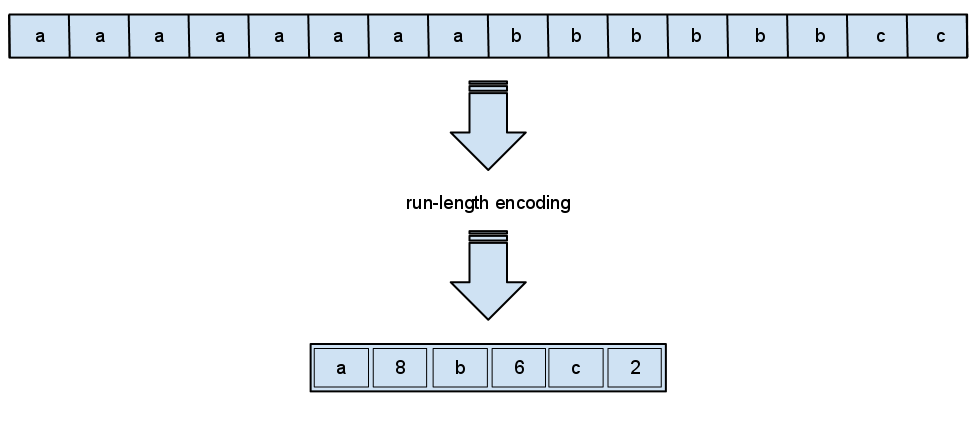
\includegraphics[width=150mm]{download.png}
	\end{figure}
	
	\subsection{Algorithm}
	a) Pick the first character from source string.\\
	b) Append the picked character to the destination string.\\
	c) Count the number of subsequent occurrences of the picked character and append the count to destination string.\\
	d) Pick the next character and repeat steps b) c) and d) if end of string is NOT reached
	
	\subsection{History and Applications}
	Run-length encoding schemes were employed in the transmission of television signals as far back as 1967.[1] It is particularly well suited to palette-based bitmapped images such as computer icons, and was a popular image compression method on early online services such as CompuServe before the advent of more sophisticated formats such as GIF.[2] It does not work well at all on continuous-tone images such as photographs, although JPEG uses it quite effectively on the coefficients that remain after transforming and quantizing image blocks.
	
	Common formats for run-length encoded data include Truevision TGA, PackBits, PCX and ILBM. The ITU also describes a standard to encode run-length-colour for fax machines, known as T.45.[3] The standard, which is combined with other techniques into Modified Huffman coding,[citation needed] is relatively efficient because most faxed documents are generally white space, with occasional interruptions of black.
	
	\section{Program}
	\begin{verbatim}
	#include<iostream>
	#include<omp.h>
	#include<string.h>
	#include<cstring>
	#include<fstream>
	#define MAX_RLEN 50
	using namespace std;
	
	char *encode(char *src)
	{
	int rlen;
	char count[MAX_RLEN];
	
	int len = strlen(src);
	char *dest = new char[2*len+1];
	
	int i,j=0,k;
	
	for(i =0;i<len;i++)
	{
	dest[j++] = src[i];
	
	rlen = 1;
	while(i+1 < len && src[i] == src[i+1])
	{
	rlen++;
	i++;
	}
	
	sprintf(count,"%d",rlen);
	
	for(k=0;*(count+k);k++,j++)
	{
	dest[j] = count[k];
	}
	}	
	dest[j] = '\0';
	return dest;
	}
	
	int main()
	{
	
	ifstream file;
	file.open("a.txt",ios::binary);
	
	string response;
	char **inp = new char*[915000];
	int i=0;
	while(getline(file,response))
	{
	inp[i] = new char[strlen(response.c_str())+1];
	strcpy(inp[i],response.c_str());
	i++;
	}
	
	int j;
	double start = omp_get_wtime();
	
	#pragma omp parallel for
	for(j=0;j<i;j++)
	{
	inp[j] = encode(inp[j]);
	//cout<<endl<<j<<endl;
	}
	cout<<"\nParallel execution : "<<omp_get_wtime() - start<<endl;
	
	
	
	start = omp_get_wtime();
	for(j=0;j<i;j++)
	{
	inp[j]=encode(inp[j]);
	}
	cout<<"\nSerial execution : "<<omp_get_wtime() - start<<endl;
	
	
	return 0;
	}
	 
	\end{verbatim}
	
	\section{Output}
	\begin{verbatim}
	altaf@altaf-ubuntu:~$ g++ -fopenmp RLE.cpp && ./a.out
	
	a1s1d1a1g1j1w4a3d1e1x6d1q1w1r1q1w1r1c1v1
	
	p1o2p1o3w1q1e1w1e1q1w4a3d1e1x6w1e1w1
	
	w4a3d1e1x6w4a3d1e1x6w4a3d1e1x6
	
	a1s1d1a1s1d1w4a3d1e1x6a1s1d1a1s1d1w4a3d1e1x6
	
	a1s1d4a1s1a4w4a3d1e1x6a1s2d3
	
	w4a3d1e1x6w4a3d1e1x6
	
	w4a3d1e1x6a11
	
	a5m1j9w1e1r1w1e1b1o1c1v2x1c1v1b1h1
	

	Parallel execution : 0.0105599
	
	
	a1s1d1a1g1j1w4a3d1e1x6d1q1w1r1q1w1r1c1v1
	
	p1o2p1o3w1q1e1w1e1q1w4a3d1e1x6w1e1w1
	
	w4a3d1e1x6w4a3d1e1x6w4a3d1e1x6
	
	a1s1d1a1s1d1w4a3d1e1x6a1s1d1a1s1d1w4a3d1e1x6
	
	a1s1d4a1s1a4w4a3d1e1x6a1s2d3
	
	w4a3d1e1x6w4a3d1e1x6
	
	w4a3d1e1x6a11
	
	a5m1j9w1e1r1w1e1b1o1c1v2x1c1v1b1h1
	
	Serial execution : 0.00838653
	
	
	\end{verbatim}
		
	\section{Conclusion:}
     Successfully implemented Run length encoding using openmp and parallelized the algorithm.
\end{document}

